% ==============================================================================
% LAB 119
% UNDERSÖKNING AV RC-KRETS
% ------------------------
%
% Author:
% Jonas Sjöberg     <tel12jsg@student.hig.se>
% Oscar Wallberg    <tco13owg@student.hig.se>
%
% License:
% Creative Commons Attribution-NonCommercial-ShareAlike 4.0 International
% See LICENSE.md for full licensing information.
% ==============================================================================

\section{Uppmätning av stegsvaret}\label{step}
% ------------------------------------------------------------------------------
Stegsvaret mäts genom att kretsen matas med en fyrkantsvåg.
% TODO: 

\subsection{Mätresultat}\label{}
% ------------------------------------------------------------------------------
% TODO:


\subsection{Simulering}\label{}
% ------------------------------------------------------------------------------
Kretsen simuleras i \texttt{Qucs} enligt Figur~\ref{fig:step-sim-step} och
Figur~\ref{fig:step-sim-param}.

Figur~\ref{fig:step-sim-step} visar det enkla fallet. En fyrkantsvåg används
för att illustrera hur kretsen svarar mot plötsliga förändringar. Grafen visar
spänningen vid punkten \texttt{Vout} som en funktion av tid.

Figur~\ref{fig:step-sim-param} visar samma skeende då värdet av $C_1$ sätts
till några av vanligt förekommande värden (standardiserade i \texttt{IEC
60063:1963}) genom en ''\emph{parameter sweep}``.  \par 
Värden av $C_1$: \SI{10}{\nano\farad},  \SI{100}{\nano\farad},
                 \SI{220}{\nano\farad}, \SI{470}{\nano\farad}, 
                 \SI{1}{\micro\farad},  \SI{2.2}{\micro\farad} 
             och \SI{4.7}{\micro\farad}.


\begin{figure}[ht]\label{fig:step-sim-step}
  \centering
  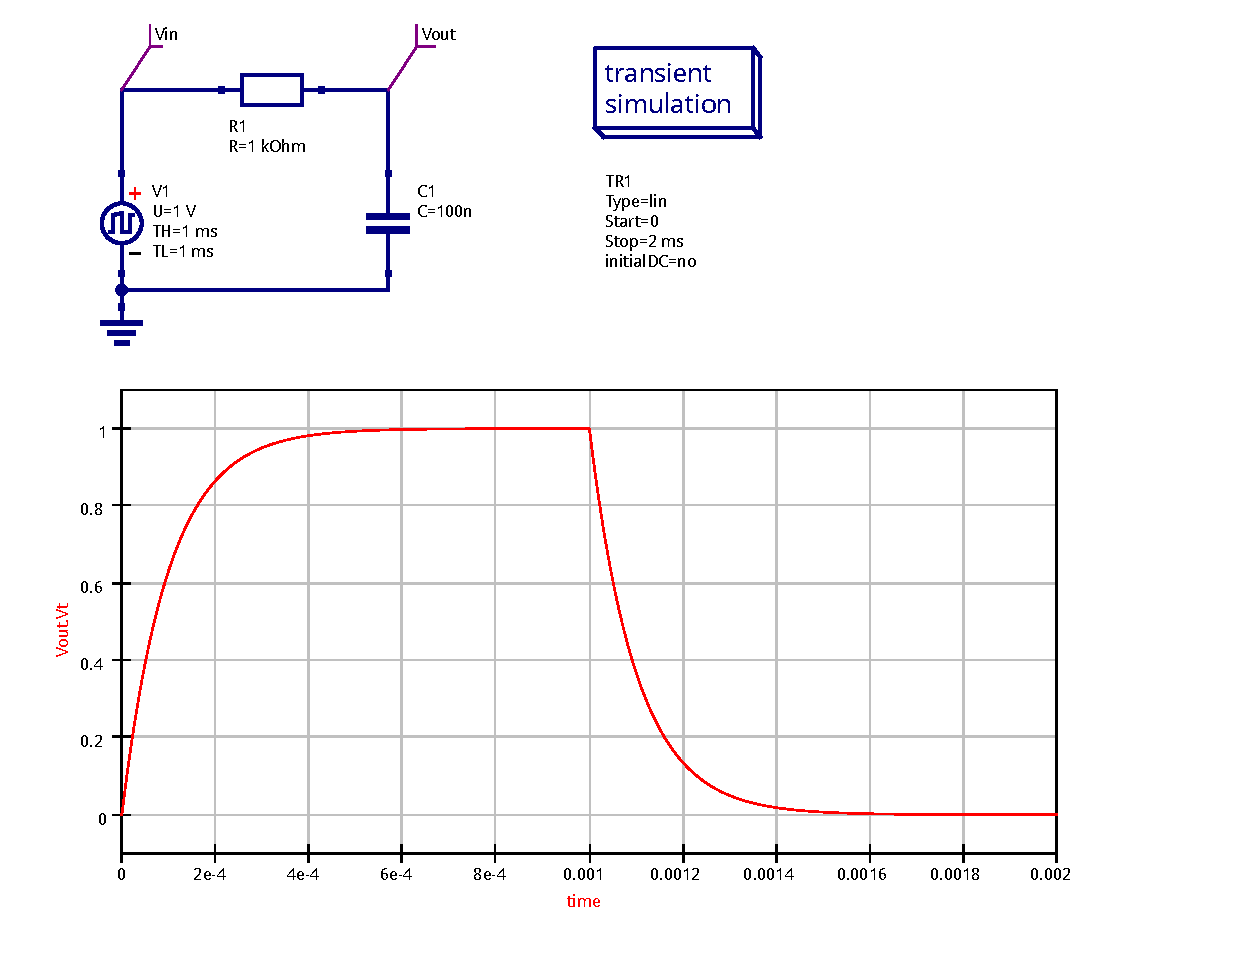
\includegraphics[width=\linewidth]{sim/ee466_lab-4_prj/uppgift-2_step}
  \caption[] {Simulering av kretsens stegsvar.}
\end{figure}

\begin{figure}[ht]\label{fig:step-sim-param}
  \centering
  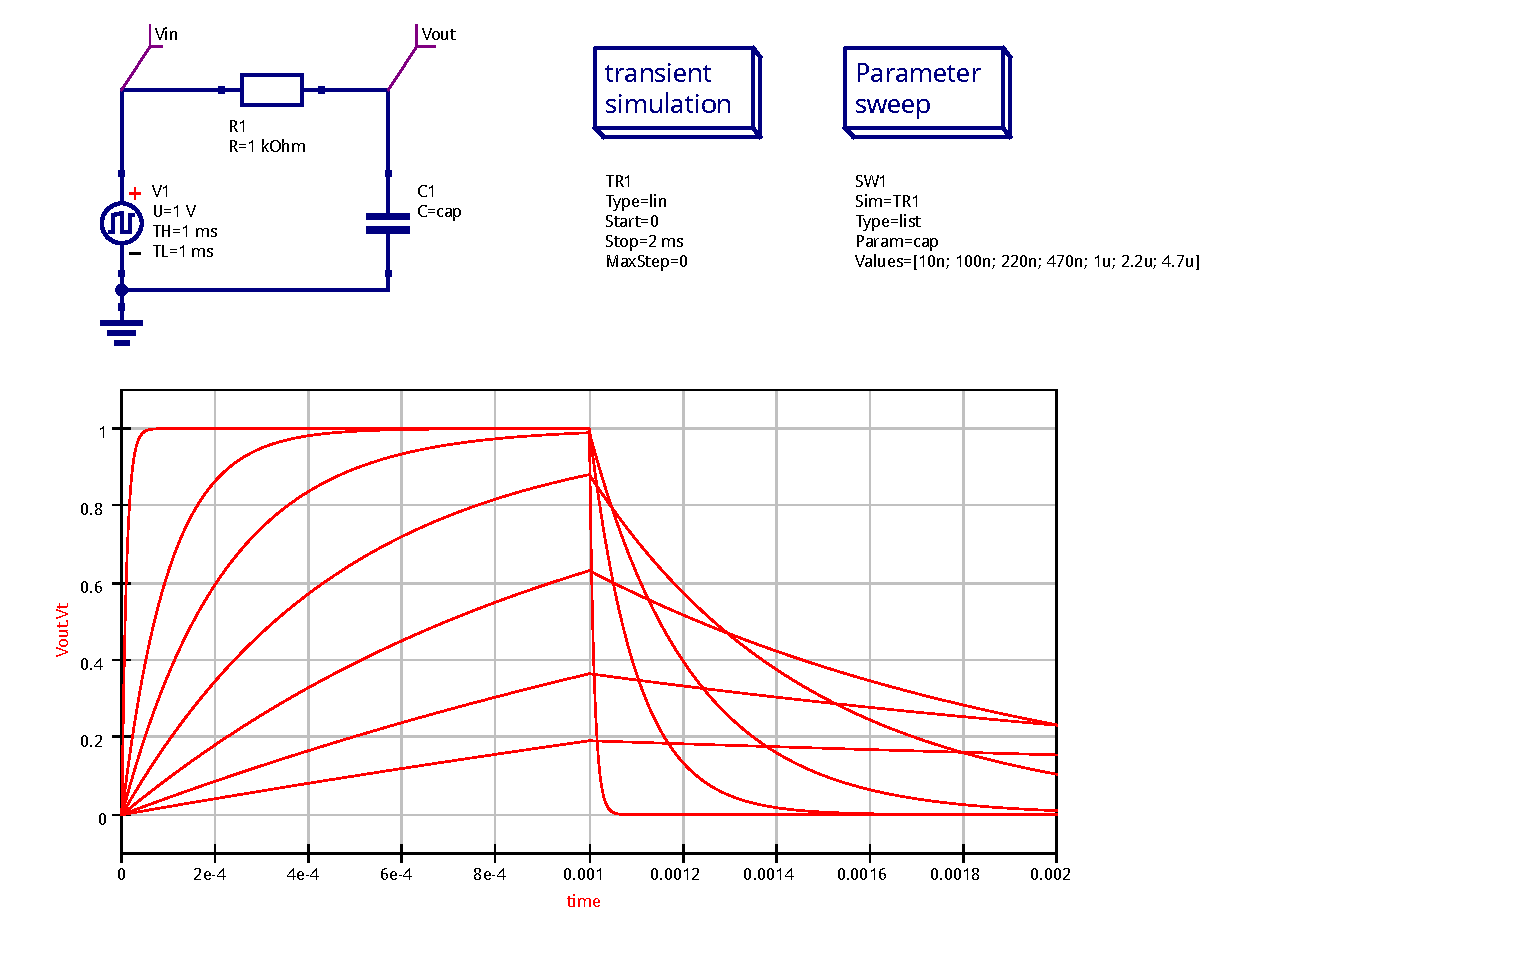
\includegraphics[width=\linewidth]{sim/ee466_lab-4_prj/uppgift-2_param}
  \caption[] {Simulering av kretsens stegsvar för olika värden av $C_1$.}
\end{figure}


\subsection{Kommentar}\label{}
% ------------------------------------------------------------------------------
% TODO:

